\documentclass[usenames,dvipsnames]{beamer}


\usetheme{Madrid}
\usecolortheme{dolphin}
\setbeamercolor{title}{fg=NavyBlue}
\setbeamercolor{frametitle}{fg=NavyBlue}
\setbeamercolor{section in toc}{fg=NavyBlue}

%\AtBeginEnvironment{theorem}{%
%	\setbeamercolor{block title}{fg=white,bg=NavyBlue}
%}

\usepackage{amsthm}
\usepackage{graphicx}
\usepackage[utf8x]{inputenc}
\usepackage{mathtools}
\mathtoolsset{showonlyrefs}
\usepackage{appendixnumberbeamer}
\usepackage{enumitem}
\usepackage{centernot}
\usepackage{tikz}
\usepackage[lined]{algorithm2e}
\usepackage{caption}
\usetikzlibrary{positioning}
\setitemize{label=-, leftmargin=*}
\usepackage{booktabs}

\DeclarePairedDelimiter{\abs}{\lvert}{\rvert}
\DeclarePairedDelimiter{\norm}{\|}{\|}
\renewcommand{\Pr}{\mathbb{P}}
\newcommand{\R}{\mathbb{R}}
\newcommand{\Var}{\operatorname{Var}}
\newcommand{\E}{\operatorname{\mathbb{E}}}
\newcommand{\iid}{\ensuremath{\stackrel{\text{iid}}{\sim}}}
\renewcommand{\phi}{\varphi}
\renewcommand{\theta}{\vartheta}
\newcommand{\epl}{\varepsilon}

% Theorem blocks
\newenvironment<>{greenblock}[1][]{%
\setbeamercolor{block title}{fg=white,bg=ForestGreen}%
\begin{block}#2{#1}}{\end{block}}
\newenvironment<>{redblock}[1][]{%
\setbeamercolor{block title}{fg=white,bg=red!75!black}%
\begin{block}#2{#1}}{\end{block}}
\newenvironment<>{orangeblock}[1][]{%
\setbeamercolor{block title}{fg=white,bg=orange!75!black}%
\begin{block}#2{#1}}{\end{block}}

% Add numbers and take out navigation symbols
\setbeamertemplate{footline}[frame number]
\beamertemplatenavigationsymbolsempty

% Text starts always from the top of the frame
\newenvironment{frameT}{\begin{frame}[t]}{\end{frame}}

\title{Random time steps geometric integrators of ordinary differential equations for uncertainty quantification of numerical errors}
\author{Assyr Abdulle, \underline{Giacomo Garegnani}}
\date{Swiss Numerics Day, 20 April 2018}
\institute[EPFL]{
\includegraphics[width=3cm]{Logo}}

%\AtBeginSection[]
%{
%	\begin{frame}<beamer>
%	\thispagestyle{empty}
%	\frametitle{Outline}
%		\tableofcontents[currentsection]
%	\end{frame}
%	\addtocounter{framenumber}{-1}
%}


\begin{document}
	
\thispagestyle{empty}
\frame{\titlepage}

\addtocounter{framenumber}{-1}

\begin{frame}
	\thispagestyle{empty}
	\frametitle{Outline}
	\tableofcontents
\end{frame}

\addtocounter{framenumber}{-1}

\section{Motivation}

\begin{frameT}
	\frametitle{Probabilistic methods -- why?}
	
	Consider Lorenz equation (atmospheric convection)
	\begin{align*}\label{eq:Lorenz}
		x' &= \sigma(y - x),  &&x(0) = -10,\\
		y' &= x(\rho - z) - y,  &&y(0) = -1,\\
		z' &= xy - \beta z,  &&z(0) = 40.
	\end{align*}
	For $\rho=28$, $\sigma=10$, $\beta=8/3$ {\color{BrickRed} chaotic behaviour}.
	
	\vspace{0.2cm}
	$\implies$ Numerical integration gives {\color{BrickRed} unreliable solutions}.
	
	\vspace{1cm}
	\only<2>{
	\begin{greenblock}[Goal]
		Establish a probability measure over the numerical solution given by classical methods.
	\end{greenblock}
	}

\end{frameT}

\begin{frameT}
	\frametitle{Probabilistic methods -- why?}
	
	\begin{figure}
		\begin{center}
			\hspace{-0.15cm}\includegraphics[width=\linewidth]{Lorenz}
		\end{center}
	\end{figure}	

	Time evolution of the first component of Lorenz equation \\
	\makebox[2cm]{\textbf{Black line}} $\to$ deterministic solution \\
	\makebox[2cm]{\color{gray} Gray lines} $\to$ family of perturbed solutions. 
	
	\only<2>{\vspace{0.5cm}
	{\color{BrickRed}Chaotic behaviour appears frequently in nonlinear differential equations.}
	}
\end{frameT}

%%%%%%%%%%%%%%%%%%%%%%%
% Probabilistic methods for ODEs

\section{Probabilistic methods for ODEs}

\begin{frame}
	\frametitle{Notation}
	Autonomous dynamical system, function $f\colon\R^d\to\R^d$ and the ODE
	\begin{equation}
	y' = f(y), \quad y(0) = y_0.
	\end{equation}
	Flow of the equation $\phi_t\colon\R^d\to\R^d$ such that
	\begin{equation}
	y(t) = {\color{ForestGreen}\phi_t(y_0)}.
	\end{equation}
	One-step method (e.g. Runge Kutta): numerical flow $\Psi_h$ such that
	\begin{equation}\label{eq:NumericalFlow}
	y_{n+1} = {\color{NavyBlue}\Psi_h(y_n)}.
	\end{equation}
\end{frame}

\begin{frame}
	\frametitle{Probabilistic methods for ODEs}
	
	\only<1>{
		{\color{ForestGreen} Filtering} methods for ODEs: fix a prior on $y(t)$ (Gaussian process), update with evaluations of $f(y)$ \cite{KeH16, CCC16}
	}
	
	\only<2>{
		{\color{ForestGreen!20} Filtering} {\color{black!20} methods for ODEs: fix a prior on $y(t)$ (Gaussian process), update with evaluations of $f(y)$ \cite{KeH16, CCC16}}
	}
	
	\vspace{1cm}
	{\color{NavyBlue} Randomised} methods for ODEs: random perturbation of deterministic numerical solutions $\to$ sampling
	\begin{itemize}
		\item Additive noise \cite{CGS16},
		\item Random time steps \cite{AbG18}.
	\end{itemize}
\end{frame}

\begin{frameT}
	\frametitle{Additive noise method}
	
    Stochastic process $\{Y_n\}_{n=1, 2, \ldots}$ with recurrence
	\begin{equation}
		Y_{n+1} = \underbrace{\Psi_h(Y_n)}_{\text{{\color{ForestGreen} deterministic}}} + \underbrace{\xi_n(h)}_{\text{{\color{NavyBlue} random}}}.
	\end{equation}
	{\color{BrickRed} Main assumption}: $\{\xi_n\}_{n=0,1,\ldots}$ iid such that for $p > 1$ and $Q \in \R^{d\times d}$
	\begin{equation}
		\E\xi_n(h) = 0, \quad \E \xi_n(h) \xi_n(h)^T = Qh^{2p+1}.
	\end{equation}
	
	\only<2>{
	\begin{greenblock}[Properties]
		If $\Psi_h$ is of order $q$ and for $\Phi\colon\R^d\to\R$ smooth
		\begin{itemize}
			\item Strong convergence: $\E\norm{y(hn)-Y_n} \leq Ch^{\min\{p, q\}}$,
			\item Weak convergence: $\abs{\Phi\big(y(hn)\big) - \E\Phi(Y_n)} \leq Ch^{\min\{2p, q\}}$,
			\item Good qualitative behavior in Bayesian inverse problems.
		\end{itemize}
	\end{greenblock}
	}
	
	\only<3>{
	\begin{redblock}[Issues]
		\begin{itemize}
			\item Robustness: $\Psi_h(Y_{n-1}) > 0 \centernot\implies \Pr(Y_n < 0) = 0$,
			\item Geometric properties are not conserved from $\Psi_h$. For example if $I(y) = y^TSy$ and $I(\Psi_h(y_0)) = I(y_0)$
			\begin{equation}
				I(Y_1) = I(y_0) + 2\xi_0(h)^T S  \Psi_h(y_0) + \xi_0(h)^T S \xi_0(h).
			\end{equation}
		\end{itemize}
	\end{redblock}
	}
\end{frameT}

\begin{frameT}
	\frametitle{Random time steps}
	
	{\color{ForestGreen}Intrinsic noise}: Random time-stepping Runge-Kutta (RTS-RK)
	\begin{equation}
		Y_{n+1} = \Psi_{{\color{NavyBlue} H_n}}(Y_n),
	\end{equation}
	{\color{BrickRed}Main assumption}: $\{H_n\}_{n=0,1,\ldots}$ iid such that for $h, C > 0$ and $p > 1$
	\begin{equation}
		H_n > 0 \text{ a.s.}, \quad \E H_n = h, \quad \Var H_n = Ch^{2p}.
	\end{equation} 
	Example: $H_n \iid \mathcal{U}(h-h^p, h+h^p)$.
	
	\only<2>{
		\begin{greenblock}[Properties]
			If $\Psi_h$ is of order $q$ and for $\Phi\colon\R^d\to\R$ smooth
			\begin{itemize}
				\item Strong convergence: $\E\norm{y(hn)-Y_n} \leq Ch^{\min\{p-1/2, q\}}$,
				\item Weak convergence: $\abs{\Phi\big(y(hn)\big) - \E\Phi(Y_n)} \leq Ch^{\min\{2p - 1, q\}}$,
				\item Good qualitative behavior in Bayesian inverse problems.
			\end{itemize}
		\end{greenblock}
	}
	
	\only<3>{
		\begin{greenblock}[Properties (Geometric)]
			\begin{itemize}
				\item Conservation of (polynomial) first integrals is inherited by $\Psi_h$,
				\item Flow map is symplectic if $\Psi_h$ is symplectic, 
				\item Long-time conservation of energy in Hamiltonian systems. 
			\end{itemize}
		\end{greenblock}
	}
	
\end{frameT}

\begin{frame}
\frametitle{Numerical experiment -- Geometric properties}
Consider the perturbed Kepler equation (model for two-body problem)
\begin{equation}
\begin{aligned}
q_1' &= p_1, && p_1' = -\frac{q_1}{\norm{q}^3} {\color{BrickRed}- \frac{\delta q_1}{\norm{q}^5}}, \\
q_2' &= p_2, && p_2' = -\frac{q_2}{\norm{q}^3} {\color{BrickRed}- \frac{\delta q_2}{\norm{q}^5}}.
\end{aligned}
\end{equation}
The {\color{NavyBlue} angular momentum} is conserved (quadratic first integral)
\begin{equation}
I(p, q) = q_1p_2 - q_2p_1
\end{equation}
$\to$ employ a Gauss method (implicit midpoint rule).

\end{frame}

\begin{frameT}
\frametitle{Numerical experiment -- Geometric properties}
\only<1>{
	\begin{figure}
		\begin{center}
			\begin{tabular}{c@{\hspace{0.3cm}}c}
				\includegraphics[width=0.2\linewidth]{KeplerOne} & \includegraphics[width=0.2\linewidth]{KeplerTwo} \\
				\includegraphics[width=0.2\linewidth]{KeplerOneAdd} & \includegraphics[width=0.2\linewidth]{KeplerTwoAdd} \\
			\end{tabular}
		\end{center}
	\end{figure}
	{\color{NavyBlue} RTS-RK} (first row), {\color{ForestGreen} Additive noise} (second row). Time $0 \leq t \leq 200$ and $200 \leq t \leq 400$ (left and right)
}
\only<2>{
	\begin{figure}
		\hspace{-0.5cm}\includegraphics[width=0.8\linewidth]{KeplerMom}
	\end{figure}
	Conservation of the {\color{NavyBlue} angular momentum} (quadratic first integral)
}
\end{frameT}


\section{Bayesian inverse problems}

\begin{frameT}
	\frametitle{Bayesian inverse problems}
	
	\begin{greenblock}[Goal] Given $\theta \in \R^n$, $f_\theta \colon \R^d \to \R^d$ and the ODE
		\begin{equation}
		y' = f_\theta(y), \quad y(0) = y_{0, \theta} \in \R^d,
		\end{equation}
		retrieve the true value $\theta^*$ from observations of $y(t)$, $t > 0$.		
	\end{greenblock}
	
	\only<2> {
	\vspace{0.2cm}
	{\color{BrickRed} Bayesian setting}: fix prior $\pi_{\mathrm{prior}}(\theta)$, consider the forward operator $\mathcal{G}$ and model observations as
	\begin{equation}
		\underbrace{\vphantom{\mathcal{G}(\theta^*)} \mathcal{Y}}_{ {\color{BrickRed} \text{observations}}} = 
		\underbrace{\mathcal{G}(\theta^*)}_{{\color{ForestGreen}\text{forward}}} + 
		\underbrace{\vphantom{\mathcal{G}(\theta^*)} \epl}_{{\color{NavyBlue}\text{noise}}}, 
		\quad \epl \sim \pi_{\mathrm{noise}},
	\end{equation} 	
	then the {\color{BrickRed} posterior distribution (density)} is
	\begin{equation}
		\pi(\theta \mid \mathcal{Y}) \propto \pi_{\mathrm{prior}}(\theta) \pi_{\mathrm{noise}}(\mathcal{Y} - \mathcal{G}(\theta)).
	\end{equation}
	}
\end{frameT}

\begin{frameT}
	\frametitle{Bayesian inverse problems}
	
	\vspace{1cm}
	\only<1-2>{
	The posterior $\pi(\theta \mid \mathcal{Y})$ is not computable, approximate with
	\begin{equation}
		 {\color{ForestGreen}\pi^h}(\theta \mid \mathcal{Y}) \propto \pi_{\mathrm{prior}}(\theta) \pi_{\mathrm{noise}}(\mathcal{Y} - {\color{ForestGreen}\mathcal{G}^h}(\theta)).
	\end{equation}
	}
	\only<3-4>{
	The posterior $\pi(\theta \mid \mathcal{Y})$ is not computable, approximate with
	\begin{equation}
		{\color{NavyBlue}\pi^{h, \mathrm{RTS}}}(\theta \mid \mathcal{Y}) \propto \pi_{\mathrm{prior}}(\theta) {\color{NavyBlue}\E^{\mathbf{H}}}\pi_{\mathrm{noise}}(\mathcal{Y} - {\color{NavyBlue}\mathcal{G}^{\mathbf{H}}}(\theta)),
	\end{equation}
	where $\mathbf{H} = (H_0, H_1, \ldots)$ is the vector of all time steps chosen in one run.
	}
	\only<2>{
		\begin{greenblock}[Properties]
			$\pi^h \to \pi$ for $h \to 0$ (in the Hellinger distance).
		\end{greenblock}
		\begin{redblock}[Issue]
			\begin{itemize}
				\item $\pi^h$ concentrated around values ``far'' from $\theta^{*}$ $\to$ non-predictive posterior
			\end{itemize}
		\end{redblock}
	}
	\only<4>{
		\begin{greenblock}[Properties]
			\begin{itemize}
				\item $\pi^{h, \mathrm{RTS}} \to \pi$ for $h \to 0$ (in the Hellinger distance). \cite{LST17}
				\item ``correct'' the non-predictive behaviour of deterministic approximations
			\end{itemize}
		\end{greenblock}
		\begin{orangeblock}[Warning]
			\begin{itemize}
				\item Approximation of $\E^{\mathbf{H}}\pi_{\mathrm{noise}}(\mathcal{Y} - \mathcal{G}^{\mathbf{H}}(\theta))$ is required
			\end{itemize}
		\end{orangeblock}
	}	
\end{frameT}

\begin{frame}
	\frametitle{Numerical experiment -- Bayesian inverse problems}
	Consider the Hénon-Heiles system (motion of a star around a galactic center), Hamiltonian with {\color{NavyBlue} energy}
	\begin{equation}\label{eq:HamHH}
	E(p, q) = \frac{1}{2}\norm{p}^2 + \frac{1}{2}\norm{q}^2 + q_1^2q_2 - \frac{1}{3}q_2^3.
	\end{equation}
	Chaotic problem for certain levels of energy.
	\begin{greenblock}[Goal]
		Find posterior $\pi((p_0, q_0) \mid \mathcal{Y})$ over the initial condition from a single observation of $(p(10), q(10))$ 
	\end{greenblock}
\end{frame}

\begin{frame}
	\frametitle{Numerical experiment -- Bayesian inverse problems}
	\only<1>{
	\begin{figure}
		\begin{center}
			\begin{tabular}{c@{\hspace{0.3cm}}c}
				\includegraphics[width=0.4\linewidth]{BayesHeun} & \includegraphics[width=0.4\linewidth]{BayesHeun2} \\ 
			\end{tabular}
		\end{center}
	\end{figure}
	Posterior distributions given by {\color{BrickRed} deterministic Heun method}.}

	\only<2>{
	\begin{figure}
		\begin{center}
			\begin{tabular}{c@{\hspace{0.3cm}}c}
				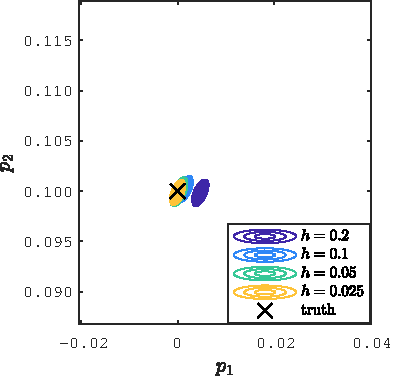
\includegraphics[width=0.4\linewidth]{BayesDet} & \includegraphics[width=0.4\linewidth]{BayesDet2} \\ 
			\end{tabular}
		\end{center}
	\end{figure}
	Posterior distributions given by {\color{NavyBlue} deterministic Störmer-Verlet method}.}

	\only<3>{
	\begin{figure}
		\begin{center}
			\begin{tabular}{c@{\hspace{0.3cm}}c}
				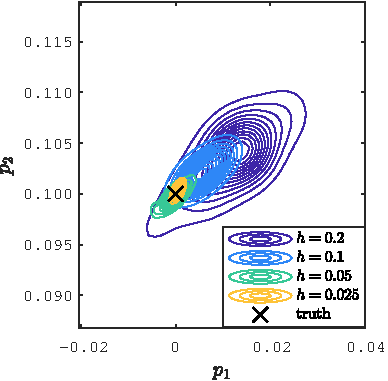
\includegraphics[width=0.4\linewidth]{BayesProb} & \includegraphics[width=0.4\linewidth]{BayesProb2} \\ 
			\end{tabular}
		\end{center}
	\end{figure}
	Posterior distributions given by {\color{ForestGreen} RTS-RK Störmer-Verlet method}.}
\end{frame}

\appendix
\begin{frame}
	\frametitle{References}
	
	\setbeamertemplate{bibliography item}[text]

	\scriptsize{
	\begin{thebibliography}{10}
		\bibitem[Abdulle and Garegnani, 2018]{AbG18}
		A. Abdulle, G. Garegnani (2018).
		\newblock Random time step probabilistic methods for uncertainty quantification in chaotic and geometric numerical integration.
		\newblock {\em preprint arXiv:1801.01340}
		
		\bibitem[Chkrebtii et~al., 2016]{CCC16}
		O.~A. Chkrebtii, D.~A. Campbell, B.~Calderhead, M.~A. Girolami (2016).
		\newblock Bayesian solution uncertainty quantification for differential	equations.
		\newblock {\em Bayesian Anal.}
		
		\bibitem[Conrad et~al., 2016]{CGS16}
		Conrad, P.~R., Girolami, M., S{\"a}rkk{\"a}, S., Stuart, A., and Zygalakis, K.
		(2016).
		\newblock Statistical analysis of differential equations: introducing
		probability measures on numerical solutions.
		\newblock {\em Stat. Comput.}
		
		\bibitem[Kersting and Hennig, 2016]{KeH16}
		Kersting, H. and Hennig, P. (2016).
		\newblock Active uncertainty calibration in {B}ayesian {ODE} solvers.
		\newblock In {\em Proceedings of the 32nd Conference on Uncertainty in Artificial Intelligence (UAI 2016)}, pages 309--318. {AUAI} Press.
		\bibitem[Lie et~al., 2017]{LST17}
		Lie, H.~C., Sullivan, T.~J., and Teckentrup, A.~L. (2017).
		\newblock Random forward models and log-likelihoods in Bayesian inverse	problems.
		\newblock {\em preprint arXiv:1712.05717}
	
	\end{thebibliography}
	}

\end{frame}

\end{document}
